\documentclass{standalone}
\usepackage{pgfplots}
\pgfplotsset{compat=newest}

\begin{document}
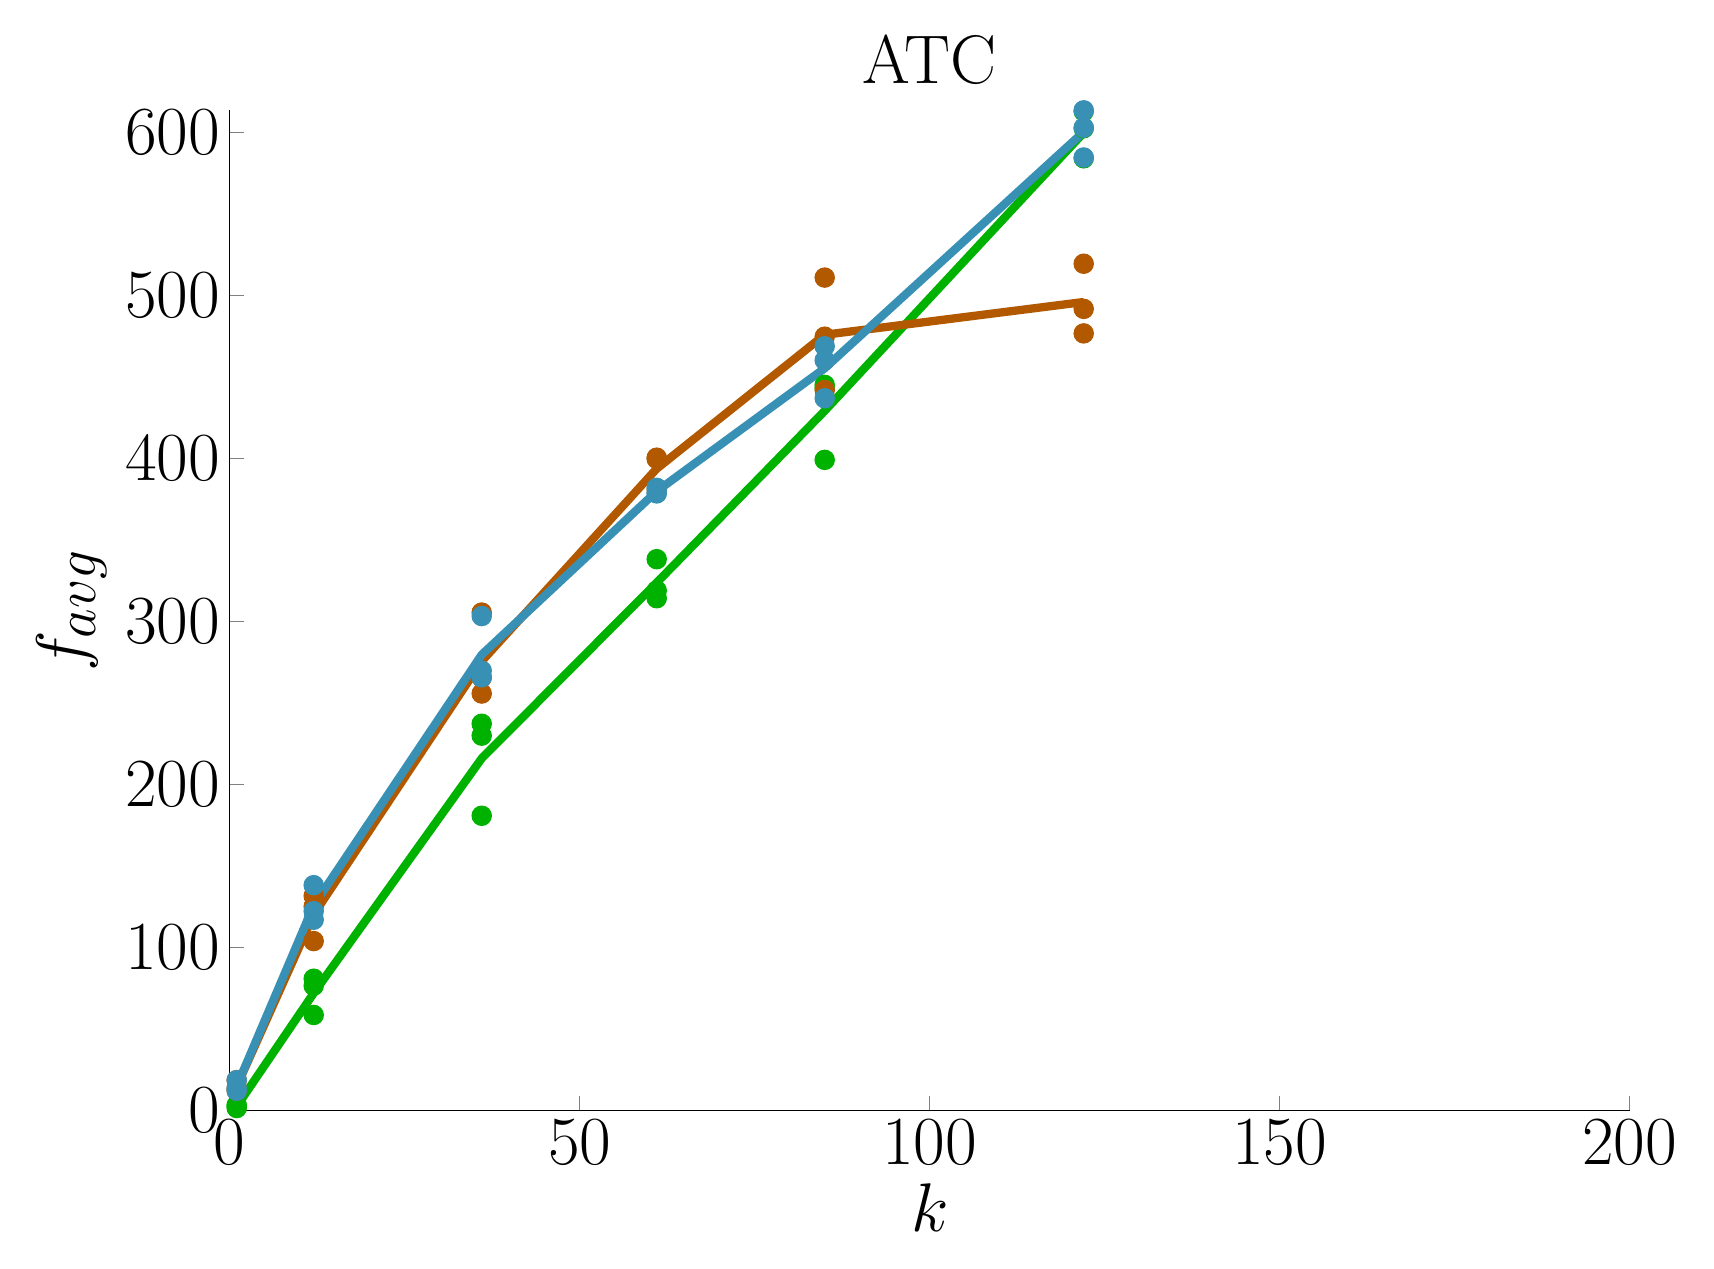
\begin{tikzpicture}

\begin{axis}[%
title style={font=\Huge},
title=ATC,
tick label style={font=\Huge},
label style={font=\Huge},
legend style={font=\Huge},
view={0}{90},
max space between ticks=50pt,
width=7in,
height=5in,
scale only axis,
xmin=0, xmax=200,
xtick={0, 50, 100, 150, 200},
xlabel={$k$},
ymin=0, ymax=613.65,
%ytick={0, 200, 400, 600, 800, 1000},
ylabel={$f_{avg}$},
major tick length=5pt,
axis lines*=left,
legend cell align=left,
clip=false]

\addplot [
only marks,
mark=*,
mark size=3.5pt,
color=green!70!black,
%solid,
%line width=2pt,
]
coordinates{
(1,1.4)(1,2.6)(1,3.2)(12,58.5)(12,76.45)(12,80.75)(36,180.75)(36,229.9)(36,237.2)(61,314.25)(61,318.95)(61,338.2)(85,399.15)(85,443.35)(85,445.15)(122,584.2)(122,602.6)(122,613.0)
};

\addplot [
only marks,
mark=*,
mark size=3.5pt,
color=orange!70!black,
%solid,
%line width=2pt,
]
coordinates{
(1,12.0)(1,13.6)(1,18.5)(12,103.85)(12,125.05)(12,131.55)(36,255.75)(36,265.5)(36,305.45)(61,381.0)(61,399.7)(61,400.5)(85,442.0)(85,474.75)(85,511.0)(122,476.75)(122,491.8)(122,519.5)
};

\addplot [
only marks,
mark=*,
mark size=3.5pt,
color=cyan!70!black,
%solid,
%line width=2pt,
]
coordinates{
(1,12.0)(1,13.6)(1,18.5)(12,116.95)(12,122.2)(12,138.15)(36,265.7)(36,269.8)(36,303.3)(61,378.55)(61,379.05)(61,382.0)(85,436.95)(85,460.25)(85,468.85)(122,584.7)(122,603.0)(122,613.65)
};

\addplot [
color=green!70!black,
solid,
line width=3pt
]
coordinates{
(1,2.4)(12,71.9)(36,215.95)(61,323.8)(85,429.216666667)(122,599.933333333)
};

\addplot [
color=orange!70!black,
solid,
line width=3pt
]
coordinates{
(1,14.7)(12,120.15)(36,275.566666667)(61,393.733333333)(85,475.916666667)(122,496.016666667)
};

\addplot [
color=cyan!70!black,
solid,
line width=3pt
]
coordinates{
(1,14.7)(12,125.766666667)(36,279.6)(61,379.866666667)(85,455.35)(122,600.45)
};


\end{axis}
\end{tikzpicture}
\end{document}
